\chapter{Analysis of existing methods}

\begin{tcolorbox}[title=Résumé du chapitre : Analyse des méthodes existantes, colframe=black!50!white]
  \paragraph{}
  Le but de ce chapitre est d'identifier les méthodes qui serviront pour la suite.

  \paragraph{}
  Le contexte mathématique et ses notations sont introduits en premier. L'objectif est de donner les
  étapes permettant de passer d'une équation aux dérivées partielles, issue du modèle physique, à une équation différentielle ordinaire, purement numérique. Pour fermer le système d'équations, les méthodes de
  discrétisation spatiale sont brièvement introduites et en particulier les deux principales du solveur CEDRE.
  Grâce à ces méthodes de discrétisation appliquées à un maillage, l'équation différentielle ordinaire finale est donc obtenue et il faut alors l'intégrer avec des méthodes d'intégration temporelle.

  \paragraph{}
  La stabilité et la notion d'ordre sont les deux principales caractéristiques nécessaires à de telles méthodes.
  Puis, les méthodes d'intégration que l'on trouve classiquement dans la littérature sont rappelées, en soulignant la dichotomie explicite/implicite.

  \paragraph{}
  Après avoir détaillé les raisons qui nous poussent à analyser les méthodes d'intégration implicite, plusieurs éléments interviennent dans la mise en place : le solveur non-linéaire, le solveur linéaire, et en particulier le passage de l'un à l'autre.
  Ce passage étant jugé insatisfaisant pour notre solveur, nous présentons la méthode JFNK, ou plus généralement une formulation sans matrice, qui s'appuie sur des parties déjà présentes de CEDRE et corrige, {\it a priori \PS{Pourquoi italique ?}}, ce défaut.
\end{tcolorbox}


  \paragraph{}
  As we aim to enhance the performances of the solver CEDRE on steady problems, we first have to define some notions.
  In particular, we need to explain what performance means.
  In this chapter, we will introduce the general problem, and the tools used to solve it.
  We will confirm some choices already made in the solver, and identify the features we would like to modify or replace.

  \section{Problem setup}

    \paragraph{}
    In order to set the mathematical framework for this study, let us start from a partial differential equation arising from the physical model, in the form of
    \begin{equation}\label{eq:pde}
      \frac{\partial \xi}{\partial t} + \operatorname{F}\left(\xi\right) = 0
    \end{equation}
    where the function $\operatorname{F}$ uses some space derivatives of the state variable $\xi$.
    This equation then describes the temporal evolution of the state variables $\xi$.

    \paragraph{}
    A particular class of such partial differential equations are conservative equations.
    They correspond to the case where the function $\operatorname{F}$ can be written as a divergence term.
    Finally, with a source term $\operatorname{S}$, those equations look like:
    \begin{equation}\label{eq:pde_conservative}
      \frac{\partial \xi}{\partial t} + \nabla \cdot \vec{\operatorname{f}}\left(\xi\right) = \operatorname{S}.
    \end{equation}
    One might notice that equation (\ref{eq:pde_conservative}) is indeed a particularisation of equation (\ref{eq:pde}), with $\operatorname{F}\left(\xi\right) = \nabla\cdot \vec{\operatorname{f}}\left(\xi\right) - \operatorname{S}$.
    Those conservative equations are the ones we will focus on in this study, as they describe the physical systems we are interested in.

    \paragraph{}
    In this work, attention is paid on computational fluid dynamics and in particular to solution of the Navier--Stokes equation and its variants: the reactive Navier--Stokes equation, the Reynold-averaged Navier--Stokes equation, etc.
    A simple form of this equation can be:
    \begin{equation}\label{eq:ns}
      \left\{\begin{aligned}
        &\partial_t\left(\rho         \right) &&+ \nabla\cdot\left( \rho \vec{u} \right) &&= 0 \\
        &\partial_t\left(\rho \vec{u} \right) &&+ \nabla\cdot\left( \rho \vec{u} \otimes \vec{u} + p \mat{\operatorname{Id}} \right) &&= \nabla\cdot \mat{\tau}\\
        &\partial_t\left( \rho E      \right) &&+ \nabla\cdot\left( \left(\rho E + p\right) \vec{u} \right) &&=
          \nabla\cdot\left( \mat{\tau} \cdot \vec{u} \right)
      \end{aligned}\right.
    \end{equation}
    with the closing relation $\rho E = \frac{p}{\gamma - 1} + \rho\frac{\vec{u} \cdot \vec{u}}{2}$.
    This relation is quite simple, as it is the one that corresponds to ideal gas with constant heat capacity.
    In the solver CEDRE, this relation is usually more complex as we are working with multifluid flows and with variable heat capacities.
    The deviatoric stress tensor $\tau$ accounts for the fluid's viscosity, and its computation depends on the model used.
    Without it, one recovers the Euler equations.
    To this simple form can be added source terms from the reactive model, source terms from the turbulence model, divergence terms from a molecular diffusion model, etc.
    Yet it is clear that with a bit of rewriting, it is possible to get back to the starting form (\ref{eq:pde}) and even the conservative form with source terms (\ref{eq:pde_conservative}).
    The quantity $\xi$ is no longer a scalar but a vector with the density $\rho$, each component of the momentum $\rho\vec{u}$ and the energy $\rho E$ as its components.
    Apart from this small change, the idea is the same.

    \paragraph{}
    When solving equations like (\ref{eq:pde}) numerically, the domain of interest is first bounded since infinite domain cannot be represented by a discrete set of variables.
    Let $\mathcal{D}$ be this computational domain.
    For a numerical computation, the different quantities, such as the state variable $\xi$, are represented discretely over the domain $\mathcal{D}$ and store it in the memory of a computer.
    To do so, the domain $\mathcal{D}$ is split into a finite number of cells, or elements, associated to the Degrees of Freedom of the solution: this is the mesh.
    Those cells are small disjoints volumes in 3D, faces in the two-dimensional space or segments in 1D, such as their union recovers the original domain.
    Interest quantities, such as the fluid velocity, density, \dots, are then stored at each node, averaged at the center of each cell or sometimes in a more complex fashion depending on the method.
    They are no longer mathematically represented by a function of the continuous physical domain $\xi: \mathcal{D} \rightarrow \mathbb{R}$ but by a finite-sized vector $\Xi$ gathering all the information across the discretised domain.
    For some simple discretisation methods, this vector consists of the quantity evaluated at the mesh nodes or averaged at the center of the cells.
    For more complex methods, this vector consists of information used to construct the solution over the domain: polynomial coefficients, spectral decomposition coefficients, etc.
    Anyway, a discretised domain is used rather than $\mathcal{D}$, the continuous one.

    \paragraph{}
    The partial differential equation (\ref{eq:pde}) transforms then into an ordinary differential equation:
    \begin{equation}
      \frac{\mathrm{d} \Xi}{\mathrm{d} t} - \operatorname{G}\left(\Xi\right) = 0 .
    \end{equation}
    The difference here is that the function $\operatorname{G}$ is a function of a discrete vector whereas $\operatorname{F}$ was a function of continuous state variables that are in turn functions of the space variable, and therefore $\operatorname{G}$ does not use any spatial derivatives.
    The negative sign is here so that this new equation is similar to the original partial differential equation (\ref{eq:pde}) and the new equation can be written in the form that corresponds to most of the literature:
    \begin{equation}\label{eq:ode}
      \frac{\mathrm{d} \Xi}{\mathrm{d} t} = \operatorname{G}\left(\Xi\right) .
    \end{equation}
    Thanks to the spatial discretisation method, the only derivative remaining is with regard to time.
    The rest is then up to the temporal integration method, which is the main topic of this thesis.
    This integration method will works on equation (\ref{eq:ode}) no matter where the function $\operatorname{G}$ comes from, but sometimes understanding the origin of this function can help so we will now introduce the spatial discretisation method used in our solver.


  \section{Brief introduction to the spatial integration schemes}

    \paragraph{}
    A \emph{spatial discretisation method} is what tells how to represent a quantity over a discretised domain, and how to compute the spatial derivative of this quantity from this representation.
    Indeed, before solving equation (\ref{eq:pde}), one must decide how to transform the continuous model into a discretised one.
    We also have to look at how the spatial derivatives arising from equation (\ref{eq:pde}) translate in the discretised model.

    \subsection{The Finite Volume method}

      \paragraph{}
      The spatial discretisation method used in the fluid solver CHARME is called the Finite Volume method \cite{EymardGallouetHerbin2000, Leterrier2003}.
      This method is particularly well fitted for conservative equations such as equation (\ref{eq:pde_conservative}).
      Such equation has the property that the quantity $\xi$ is conserved: without source terms, the variation of the total quantity $\xi$ over the domain $\mathcal{D}$ is equal to the flux $f\left(\xi\right)$ coming through the boundary $\partial\mathcal{D}$.
      In the case of the Navier--Stokes equations (\ref{eq:ns}), the density, the momentum and the energy are conserved throughout time, apart from what comes in and out of the domain.
      In a close domain where nothing comes in or out, they are indeed conserved.
      The main interest of the Finite Volume method is that this property stays true through the spatial discretisation step.

      \paragraph{}
      The Finite Volume method consists in integrating the partial differential equation over each cell of the mesh.
      Writing $\mathcal{V}_i$ the volume of the $i$th cell:
      \begin{equation}
        \int_{\mathcal{V}_i} \frac{\partial \xi}{\partial t} \mathrm{d}v + \int_{\mathcal{V}_i} \nabla\cdot \vec{\operatorname{f}}\left(\xi\right) \mathrm{d}v = \int_{\mathcal{V}_i} \operatorname{S} \mathrm{d}v .
      \end{equation}
      Then the Green--Ostrogradski theorem transforms the flux divergence into a surface integral:
      \begin{equation}
        \frac{\mathrm{d}}{\mathrm{d} t} \int_{\mathcal{V}_i} \xi\mathrm{d}v + \oint_{\partial\mathcal{V}_i} \vec{\operatorname{f}}\left(\xi\right) \cdot \vec{\mathrm{d}s} = \int_{\mathcal{V}_i} \operatorname{S} \mathrm{d}v .
      \end{equation}
      By writing $\square_i = \frac{1}{\norm{\mathcal{V}_i}} \int_{\mathcal{V}_i} \square \mathrm{d}v$ the average in the $i$th cell, it comes:
      \begin{equation}
        \frac{\mathrm{d}\xi_i}{\mathrm{d} t}  + \frac{1}{\norm{\mathcal{V}_i}} \oint_{\partial\mathcal{V}_i} \vec{\operatorname{f}}\left(\xi\right) \cdot \vec{\mathrm{d}s} = \operatorname{S}_i .
      \end{equation}

      \paragraph{}
      As stated before, the spatial discretisation method does transform the partial differential equation into an ordinary differential equation.
      It tells to store quantities as their averaged values represented at the center of gravity of each cell as the vector $\Xi$.
      An important aspect concerns the transformation of the divergence from equation (\ref{eq:pde_conservative}) into a flux surface average, and the flux computation is still here an open question.
      The mesh cells are supposed to be polyhedrons and they have a finite number of planar faces.
      The integral over the boundary of the cell can be decomposed by the faces, to get the approximation:
      \begin{equation}
        \oint_{\partial\mathcal{V}_i} \vec{\operatorname{f}}\left(\xi\right) \cdot \vec{\mathrm{d}s} \approx \sum_{j\textrm{ neighbor of } i} \vec{\operatorname{f}}_{ij} \cdot \vec{s_{ij}}
      \end{equation}
      where $\vec{s_{ij}}$ is the product of the face area and the unit normal vector directed outwards volume $i$ and $\vec{\operatorname{f}}_{ij} \cdot \vec{s_{ij}}$ is an approximation of the flux going through the face between cells $i$ and $j$.
      This approximation is a key element of the Finite Volume method and will be discussed later.
      The function $\operatorname{G}$ from equation (\ref{eq:ode}) can now be computed: for each face of the mesh, one computes $\vec{\operatorname{f}}_{ij} \cdot \vec{s_{ij}}$, adds this value to the $i$th component and removes it from the $j$th component of the new vector.
      Then, after adding the source terms, this yields the vector containing the result of $\operatorname{G}\left(\Xi\right)$.
      As can be seen, every contribution of the flux added in a cell is removed from another, and therefore this spatial discretisation method preserves the conservation of the underlying equation.


    \subsection{The Riemann problem}

      \paragraph{}
      The last remaining problem with this presentation of the Finite Volume method is how to compute the flux going through cell interfaces.
      On the interfaces between two cells, the left and right quantities $\xi_L$ and $\xi_R$ are known and are used to compute the corresponding flux.
      It is possible here to use a reconstruction method to get a better approximation of the quantities at the left and right sides of the interface, and therefore the left and right quantities at the face $\xi_L^*$ and $\xi_R^*$ are used, rather than the quantities at the cell center.
      The idea is now to compute the flux going through the face as a function of $\xi_L^*$, $\xi_R^*$ and the surface vector $\vec{s}$.
      From the interface point of view, there are two possible different states, one from each side: this is what is called a Riemann problem.
      A Riemann problem is an initial value problem applied to a conservation equation, where the initial solution is piecewise constant with a single possible discontinuity.
      By working with the equation and deriving the jump condition, it is possible to compute the quantity from a possibly discontinuous state at the interface.
      Then it is possible to evaluate the flux associated with this state going through the surface.
      This approach can be called the exact Riemann solver as it uses the exact solution of the Riemann problem.
      But the drawback of this approach usually is the computational cost required to find this exact solution and people generally revert to approximate Riemann solvers, compromising between speed and accuracy.
      Several approximate Riemann solvers are available to the user in our solver, such as the well known Roe, HLLC or AUSM+ schemes \cite{Roe1981, Toro2009}.


    \subsection{Gradient reconstruction methods}

      \paragraph{}
      The standard Finite Volume method represents quantities with the averaged value in each cell.
      This corresponds to a first-order discretisation method.
      Simply put, it means that it can represent quantities exactly as 0-order polynomials locally to each cell.
      There are ways to achieve higher-order representation such as with the MUSCL approach \cite{VanLeer1979}.
      It consists in handling the surface flux evaluation as explained in the Riemann problem part on one hand, and deciding what left and right quantities to feed to this flux computation on the other hand.
      In our solver, there are two ways to construct high-order states to give to the flux computation method.
      They are described in the following parts.
      For both of them, the idea is to use neighbouring data to enhance the order of the local representation.


      \subsubsection{The $k$-exact method}

        \paragraph{}
        The first method used to reconstruct high-order quantities is called the \emph{$k$-exact} method with successive corrections.
        The idea is to construct iteratively an order $k$ representation of the quantity using the neighbouring order $k-1$ representation \cite{HaiderCroisilleCourbet2009}.
        This method is often employed to achieve a second-order reconstruction, as choose most users, but it can also achieve higher-order reconstructions \cite{HaiderCroisilleCourbet2011, HaiderCourbetCroisille2018, PontBrennerCinellaEtAl2017}.
        At each step, while increasing the order of the representation, it is important not to create a local maximum or minimum.
        This might happen close to discontinuities in the solution, or near rapidly varying spots.
        It is indeed common, when interpolating, to create local overshoot or undershoot.
        One might think here about Gibbs or Runge's phenomena, and despite the problem here being a different one, the idea is the same.
        Creating local extrema in the solution can be troublesome, and so the $k$-exact method includes limiters to limit reconstructed data.


      \subsubsection{The Multislope method}

        \paragraph{}
        The second method used to reconstruct high-order quantities is called the \emph{Multislope} method.
        This method is a direct adaptation of the structured directional method to unstructured grids.
        It consists in defining local directions for the interpolation of the unknown on the face.
        For a given cell and one of its face, one can draw the line from their centers.
        Information is interpolated on this line using neighbouring cells to get the local slope.
        The mechanism to define the slopes and the geometric treatment is quite complex and it won't be discussed here.
        The details are provided in \cite{LeTouzeMurroneGuillard2015}.
        Finally, the Multislope method gives a second-order reconstruction.
        Once again, this reconstruction might create local maxima or minima, and therefore it uses slope limiters \cite{Venkatakrishnan1993, BergerAftosmis2005} to prevent it.


      \paragraph{}
      We briefly explained above the spatial discretisation method used in our solver, as it might help the analysis of the time integration part.
      The Finite Volume method averages the partial differential equation over each cell of the mesh, which transforms the flux divergence into a flux surface average.
      A reconstruction method, the $k$-exact method or the Multislope method, is then used to get a higher-order representation of the solution so that the surface flux can be computed at each face.
      Slope limiters are used to prevent the formation of local extrema, which can be harmful to the computation.
      The choices made for the spatial discretisation methods are motivated by the fact that CEDRE and in particular the fluid solver CHARME aim to work with general unstructured meshes.
      It restricts the choices of algorithms, as handling general unstructured meshes can prove difficult for simple spatial discretisation methods.
      It means that the methods must be more robust, which often means less precise.


  \section{Introduction to the time integration methods}

    \paragraph{}
    With the help of a spatial discretisation method, the equation to solve is now an ordinary differential equation.
    The main objective of this thesis is focused on the resolution of steady problems.
    The steady solution of equation (\ref{eq:ode}) is given by $\operatorname{G}\left(\Xi\right) = 0$.
    To get the solution, one might then try to find a root of the function $\operatorname{G}$.
    Unfortunately, with our typical applications, this function $\operatorname{G}$ has got bad mathematical properties, such as its stiffness, arising from the nonlinearities of the underlying equations.
    Therefore, algorithms that try to find a root of $\operatorname{G}$ struggle and usually fail.
    Another approach is to take an initial value $\Xi_0$, and to solve the equation (\ref{eq:ode}) for this initial value.
    After a long enough time, one hopes that $\Xi$ will reach the desired steady solution.

    \paragraph{}
    The idea is now to solve the temporal evolution of $\Xi$ to get the solution after a long time when it approaches the steady solution.
    The equation is solved numerically, which means the next solution is computed iteratively after a given time step, knowing the current one.
    It is also possible to modify the equation, as the interest is in the final state, not in the transient one.
    It is possible, for example, to use local time-stepping, which consists in having each cell of the mesh move forward in time with its own time step.
    The resulting transient states do not make sense from a physical point of view, as the equation solved is not the initial one, but it converges to the same steady solution.
    Therefore, it is alright to change the equation as long as it gives the same steady solution.
    Finally, this way of finding a converged steady solution is what is called a \emph{Pseudo-Transient Continuation} method \cite{KelleyKeyes1996}.

    \paragraph{}
    After deciding on an initial value, the equation to solve is:
    \begin{equation}\label{eq:init_value_ode}
      \left\{\begin{aligned}
        & \frac{\mathrm{d} \Xi}{\mathrm{d}t} = \operatorname{G}\left(\Xi\right) \\
        & \Xi\left(t_0\right) = \Xi_0
      \end{aligned}\right. .
    \end{equation}
    A time integration method is going to produce a succession of solutions: starting from $\Xi_0$, it produces $\Xi_1$ at $t_1$, then $\Xi_2$ at $t_2$, and $\Xi_n$ at $t_n$, etc.
    Let $\Delta t_n$ be the time step $t_{n+1} - t_n$.
    The following is related to a single step of the time integration method, so the subscript on the time step can be drop as it is not meaningful.
    For a steady problem, the evolution of the solution has no interest and it seems reasonable to want to "go fast" to the steady state, meaning to use as large a time step as possible.
    Unfortunately, not every time integration method allows large time steps due to the well-known Courant--Friedrichs--Lewy condition \cite{CourantFriedrichsLewy1967}.
    Some tools must be defined in order to help decide on the method to use.


    \subsection{Analysis of time integration methods}

      \subsubsection{Consistency and order}

        \paragraph{}
        A time integration method must respect some properties to be "well-behaved".
        For instance, it has to be consistent.
        To define the consistency, let us look at equation (\ref{eq:init_value_ode}).
        After one step, a numerical method gives a value $\Xi_1$, believed to be near the exact value $\Xi\left(t_0 + \Delta t\right)$.
        A numerical time integration method is said to be consistent if:
        \begin{equation}
          \lim_{\Delta t \rightarrow 0} \frac{\Xi_1 - \Xi\left(t_0 + \Delta t\right)}{\Delta t} = 0 .
        \end{equation}
        Also, the method is of order $p$ if the local error is in $\Delta t^{p+1}$ \cite{Iserles2008}:
        \begin{equation}
          \Xi_1 - \Xi\left(t_0 + \Delta t\right) = O\left(\Delta t^{p+1}\right) .
        \end{equation}
        This means a $p$-order method can recover exactly a solution that is a polynomial function of time with an order less or equal to $p$.

        \paragraph{Note:}
        The order of a time integration method reflects its "local" behaviour, meaning on a single given time step, provided it is small enough.
        In the field of spatial discretisation of partial differential equations, the order $p$ of a method is such as:
        \begin{equation}
          \norm{\Xi - \Xi_{exact}} = O\left(h^p\right)
        \end{equation}
        where $h$ is the spatial discretisation parameter.
        There is a difference between the two definitions: the error order of magnitude is $p+1$ for the temporal method and $p$ for the spatial one.
        This is due to the fact that the error in the spatial case is global: it sums the error over the whole domain.
        It would correspond to counting the error on each step for the temporal integration.
        To convince oneself, one could say that when solving the differential equation on an interval $\left[0, T\right]$ with a fixed $T$, the global error of a $p$-order method would behave as $O\left(\Delta t^p\right)$ as it amounts to summing $T/\Delta t$ local errors of $O\left(\Delta t^{p+1}\right)$.
        The coherency with the definition of the order for spatial discretisation methods is now clear.
        If this trick can help understand the difference between the two definitions, this is indeed just a mental trick and not a rigorous mathematical proof.
        To get this proof, more hypotheses on the method are required \cite{Iserles2008}.


      \subsubsection{Stability}

        \paragraph{}
        A meaningful criterion in the choice of a time integration method is stability.
        Depending on the application, different levels of stability are expected in order to avoid a numerically induced divergence of the computation.

        \paragraph{}
        The stability of a time integration method is usually analysed on the ordinary differential equation with a linear right-hand side \cite{HairerWanner1996}.
        The reason is that if $\tilde{\Xi}$ is solution of equation (\ref{eq:init_value_ode}), $\operatorname{G}$ can be linearised in $\tilde{\Xi}$.
        With $y = \Xi - \tilde{\Xi}$ and $J = \frac{\partial \operatorname{G}}{\partial \Xi}\left(\tilde{\Xi}\right)$, assumed constant, it comes:
        \begin{equation}\label{eq:dahlquist}
          \frac{\mathrm{d} y}{\mathrm{d} t} = J y .
        \end{equation}
        This new equation used to analyse the stability of time integration methods is the one called the Dahlquist test equation.
        This equation is studied in $\mathbb{C}$, so that eigenvalues and eigenvectors of the matrix $J$ exists.

        \paragraph{Note:}
        When looking at a method applied to the Dahlquist test equation (\ref{eq:dahlquist}), it is assumed that the real parts of the eigenvalues of $J$ are all negative.
        This choice may seem arbitrary but can be understood with the following example.
        Let us work in $\mathbb{C}^2$, with:
        \begin{equation}
          J = \begin{pmatrix} -1 & 0 \\ 0 & 10^3 \end{pmatrix}, \quad y_0 = \begin{pmatrix} 1 \\ 0 \end{pmatrix} .
        \end{equation}
        The solution of the equation is then:
        \begin{equation}
          y\left(t\right) = \begin{pmatrix} e^{-t} \\ 0 \end{pmatrix} .
        \end{equation}
        As the equation is solved numerically, the floating point representation introduces some roundoff error.
        The initial condition may then be
        \begin{equation}
          y_0' = \begin{pmatrix} 1 \\ \epsilon \end{pmatrix}
        \end{equation}
        instead of the exact one $y_0$, with a typical $\epsilon = 10^{-15}$ for double precision.
        Let us suppose that we have an exact time integration method that gives the exact solution at each time step $t_n = n\Delta t$.
        The solution computed by this method will be:
        \begin{equation}
          y_n = \begin{pmatrix} e^{-n\Delta t} \\ \epsilon e^{10^3 n \Delta t} \end{pmatrix}
        \end{equation}
        that gives an error of $\epsilon e^{10^3 n\Delta t}$.
        For the numerical values suggested here, this amount to an error as large as $10^6$ for $n = 5$ and $10^{28}$ for $n = 10$.
        The explosion of the error comes from the fact that the positive eigenvalue of $J$ amplifies the roundoff error.
        This phenomenon has nothing to do with the time integration scheme, but with the equation.
        Finally, this is why equation (\ref{eq:dahlquist}) is studied assuming the eigenvalues of $J$ are negative.

        \paragraph{Single-step methods}
        To compute the solution at the next time step, some methods need only to know the current solution.
        Such methods are called single-step methods.
        A single-step method applied to the Dahlquist test equation (\ref{eq:dahlquist}) leads to the following relationship between the current solution and the next one:
        \begin{equation}\label{eq:single_step}
          y_{n+1} = g\left(\Delta tJ\right)y_n .
        \end{equation}
        For most time integration methods, $g$ is an analytic function.
        The initial value $y_0$ can be decomposed on a basis of eigenvectors of $J$, $v_1, \dots, v_N$, associated with the eigenvalues $\alpha_1, \dots, \alpha_N$: $y_0 = \sum_{i=1}^N \lambda_i v_i$.
        Because $g$ is an analytic function, it comes immediatly:
        \begin{equation}
          y_n = \sum_{i=1}^N \lambda_i g\left(\Delta t \alpha_i\right)^n v_i .
        \end{equation}
        It is now straightforward to deduce a stability condition for the single-step method: if for any $i$ there is $\left|g\left(\Delta t\alpha_i\right)\right| < 1$, then $y_n$ converges to 0.
        This is how the stability region of a time integration method is defined:
        \begin{equation}
          \left\{ \, z \in \mathbb{C} \; \mid \; \left| g\left(z\right) \right| < 1 \, \right\} .
        \end{equation}
        When each eigenvalue of $\Delta t J$ falls in the stability region, then the method is stable.

        \paragraph{}
        If an eigenvalue is not in the stability region, the associated eigendirection will be amplified and a numerical instability will lead to the divergence of the computation.
        We can see that the argument of the function $g$ is not $J$ but $\Delta t J$.
        This means that stability can be achieved by choosing wisely the time step: with a small enough $\Delta t$ one can ensures that each eigenvalue falls into the stability region.
        Unfortunately, this often forces the user to set a relatively small time step, which is an issue for steady computations.


        \paragraph{Multistep methods}
        Some methods do not fall into the previous framework.
        The multistep methods, in particular, cannot be written under the form of equation (\ref{eq:single_step}).
        These methods use not only $y_n$ to find $y_{n+1}$, but the $k$ previous steps.
        Applied to equation (\ref{eq:dahlquist}), they can be written in the form:
        \begin{equation}
          y_{n+1} = \sum_{i=1}^k g_{k-i}\left(\Delta t J\right) y_{n+1-i} .
        \end{equation}
        When looking for $y_i$ under the form $y_i \propto \mu^{i}$, one has:
        \begin{equation}
          \mu^k = \sum_{i=1}^k g_{k-i}\left(\Delta t J\right) \mu^{k-i}
        \end{equation}
        which leads to identifying the polynomial $g_{\Delta t J}\left(\mu\right) = \mu^k - \sum_{i=0}^{k-1}g_i\left(\Delta t J\right)\mu^i$.
        If each root of this polynomial is of modulus less than 1, the solution converges to 0.
        This is how the stability region for multistep methods is defined \cite{HairerWanner1996}:
        \begin{equation}
          \left\{ \, z \in \mathbb{C} \; \mid \; \parbox{25em}{all roots of $X^k - \sum_{i=0}^{k-1}g_i\left(z\right)X^i$ are of modulus less or equal to 1, strictly less to 1 for roots with multiplicity}
           \, \right \} .
        \end{equation}
        Once again, if all eigenvalue of $\Delta t J$ falls in the stability region, then the method is stable.

        \paragraph{}
        The key property resulting in the stability analysis of time integration methods is the \emph{A-stability} \cite{Dahlquist1963}.
        A time integration method is A-stable if its stability region contains the left half complex plane.
        Simply put, a method is A-stable if it converges to 0 when it should, and does not diverge due to numerical errors.
        The A-stability is interesting, as an A-stable method is also said to be unconditionally stable, whereas a method that is not is conditionally stable.
        This other characterisation comes from the fact that a non-A-stable method needs to respect some additional criteria to be stable, on the time step it uses for example, whereas an A-stable method is stable no matter the time step.
        As we said before, we would like to use large time steps to quickly find the steady state of our applications, and that is why we look for A-stability in our methods.


      \paragraph{}
      Having defined the concepts of stability and order of time integration methods, we are now equipped to analyse them.
      We see from the literature that time integration methods are usually split into two groups: explicit and inplicit methods.
      We can now look at methods from this literature, starting with the simpler explicit methods.


    \subsection{Explicit methods}

      \paragraph{}
      Explicit methods are called this way because, at each step, the computation of the next solution is straightforward: they give it explicitly as a function of currently available data.
      They are largely used in unsteady computational fluid dynamics simulations.
      Their strength comes from the fact that they are usually simple and therefore easy to implement in a solver, and computationally inexpensive compared to non-explicit methods.


      \subsubsection{Explicit Euler method}

        \paragraph{}
        The explicit Euler method is the most simple time integration method.
        It consists in integrating equation (\ref{eq:init_value_ode}) between $t_n$ and $t_{n+1}$ assuming the function $\operatorname{G}$ stays constant, equal to $\operatorname{G}\left(\Xi_n\right)$.
        Equivalently, it consists in replacing the time derivative $\frac{\mathrm{d} \Xi}{\mathrm{d} t}$ by a finite difference $\frac{\Xi_{n+1} - \Xi_n}{\Delta t}$ and evaluating $\operatorname{G}$ in $\Xi_n$.
        Then, the method gives:
        \begin{equation}
          \Xi_{n+1} = \Xi_n + \Delta t \operatorname{G}\left(\Xi_n\right) .
        \end{equation}

        \paragraph{}
        After verifying that this is a first-order method, a quick stability analysis gives a stability region equal to the open unity disk centred in -1.
        Practically, this stability region is often deemed unsatisfactory as it forces the use of small time steps.
        Yet this method is a classic that must be introduced before talking about more complex methods.


      \subsubsection{Runge--Kutta methods}

        \paragraph{}
        Instead of making one step forward in time as the explicit Euler method, Runge--Kutta methods will make a set of intermediate steps, and find the final solution as a combination of those intermediate steps.
        It starts from the value of $\Xi_n$ known in $t_n$ and given intermediates steps $t_{n, i} = t_n + c_i\Delta t$ for $1 \leq i \leq k$, with a fixed $k$.
        An exact integration between $t_n$ and $t_{n, i}$ of equation (\ref{eq:init_value_ode}) leads to:
        \begin{equation}
          \Xi\left(t_{n, i}\right) = \Xi_n + \Delta t \int_{t_n}^{t_{n,i}} \operatorname{G}\left(\Xi\left(t\right)\right) \mathrm{d}t .
        \end{equation}
        The integral on the right-hand side is then approximated with a quadrature using the previously computed intermediate steps:
        \begin{equation}
          \int_{t_n}^{t{n,i}} \operatorname{G}\left(\Xi\left(t\right)\right) \mathrm{d}t \approx \sum_{j = 1}^{i-1} a_{ij} \operatorname{G}\left(\Xi\left(t_{n,j}\right)\right) .
        \end{equation}
        Once each intermediate step is known, equation (\ref{eq:init_value_ode}) is integrated between $t_n$ and $t_{n+1}$ and the resulting integral is approximatex using the intermediate steps.

        \paragraph{}
        To sum up, a Runge--Kutta method iterates in the following way:
        \begin{equation}\label{eq:rk}
          \left\{\begin{aligned}
            \Xi_{n+1} &= \Xi_n + \Delta t \sum_{i = 1}^k b_i \operatorname{G}\left(\Xi_{n,i}\right) \\
            \textrm{with}\quad \Xi_{n,i} &= \Xi_n + \Delta t \sum_{j = 1}^{i-1} a_{ij} \operatorname{G}\left(\Xi_{n,j}\right)
          \end{aligned}\right. .
        \end{equation}

        \paragraph{}
        A Runge--Kutta method is characterised by its size $k$ and by the quadrature coefficients: $a_{ij, 1\leq j<i\leq k}$, $b_{i, 1\leq i\leq k}$ and $c_{i, 1\leq i\leq k}$.
        There are as many Runge--Kutta methods as there are choices in the quadrature coefficients, but not all choices give good methods.
        There are criteria that the coefficients must follow to ensure the consistency of the method, and then criteria with more complexity as the order increases.
        The quadrature coefficients are often arranged in the Butcher tableau:
        \begin{equation}
          \begin{array}{c|c}
            c & A \RKBar \transpose{b}
          \end{array}
          \qquad = \qquad
          \begin{array}{c|ccccc}
            0\\
            c_2    & a_{21} \\
            c_3    & a_{31} & a_{32} \\
            \vdots & \vdots &        & \ddots\\
            c_k    & a_{k1} & a_{k2} & \hdots & a_{k,k-1} \RKBar
            b_1    & b_2    & \hdots & b_{k-1} & b_k
          \end{array} .
        \end{equation}

        \begin{table}
          \center
          \begin{tabular}{M{.15\textwidth}M{.3\textwidth}M{.4\textwidth}c}
            \begin{tabular}{c|c}
              \multicolumn{1}{c}{} \\ \multicolumn{1}{c}{} \\ \multicolumn{1}{c}{} \\ 0 \RKBar 1
            \end{tabular} &
            \begin{tabular}{c|cc}
              \multicolumn{1}{c}{} \\ \multicolumn{1}{c}{} \\ 0 \\ 1/2 & 1/2 \RKBar 0 & 1
            \end{tabular} &
            \begin{tabular}{c|cccc}
              0 \\ 1/2 & 1/2 \\ 1/2 & 0 & 1/2 \\ 1 & 0 & 0 & 1 \RKBar 1/6 & 1/3 & 1/3 & 1/6
            \end{tabular} & \\[35pt]
            RK1 & RK2 & RK4 & \\
          \end{tabular}
          \caption{Butcher tableau for the explicit Euler, Midpoint and RK4 methods.}\label{tab:rk_butcher}
        \end{table}

        \paragraph{}
        The Butcher tableau of some well-known Runge--Kutta methods are shown in table \ref{tab:rk_butcher}.
        The RK1 method is in fact equivalent to the explicit Euler method.
        The RK2 method is one of the 2 steps second-order Runge--Kutta method.
        This one is also called the Midpoint method.
        The RK4 method is a fourth-order method with 4 steps.
        This is the most famous Runge--Kutta method, vastly used for explicit time integration of ordinary differential equations.

        \paragraph{}
        We note that the coefficients $c_i$ do not appear in the definition from equation (\ref{eq:rk}).
        It is because the differential equation (\ref{eq:ode}) is autonomous: the function $\operatorname{G}$ does not depends explicitly on the time.
        If it did, the equation would then be non-autonomous, and $\operatorname{G}$ would be a function of two variables: the state vector $\Xi$ and the time $t$.
        Equation (\ref{eq:rk}) becomes then:
        \begin{equation}
          \left\{\begin{aligned}
            \Xi_{n+1} &= \Xi_n + \Delta t \sum_{i = 1}^k b_i \operatorname{G}\left(\Xi_{n,i} \ ,\  t_n + c_i \Delta t\right) \\
            \textrm{with}\quad \Xi_{n,i} &= \Xi_n + \Delta t \sum_{j = 1}^{i-1} a_{ij} \operatorname{G}\left(\Xi_{n,j} \ ,\  t_n + c_j \Delta t\right)
          \end{aligned}\right. .
        \end{equation}

        \paragraph{}
        It can be shown that the order $p$ of the method is less or equal to the number of steps $k$.
        Up to 4 steps, it is possible to choose the quadrature coefficients to have $p = k$.
        Above that, getting a lower bound on the order depending on the number of steps is still an open problem as of today.
        For a Runge--Kutta method of order $p$, the corresponding function used for the stability analysis is \cite{HairerWanner1996}:
        \begin{equation}
          g\left(z\right) = 1 + z + \frac{z^2}{2} + \dots + \frac{z^p}{p!} + O\left(z^{p+1}\right) .
        \end{equation}
        When $p = k$, the last term $O\left(z^{p+1}\right)$ is in fact null.
        Figure \ref{fig:rk_stab} shows the stability region of the Runge--Kutta methods of orders up to 4.

        \begin{figure}
          \centering
          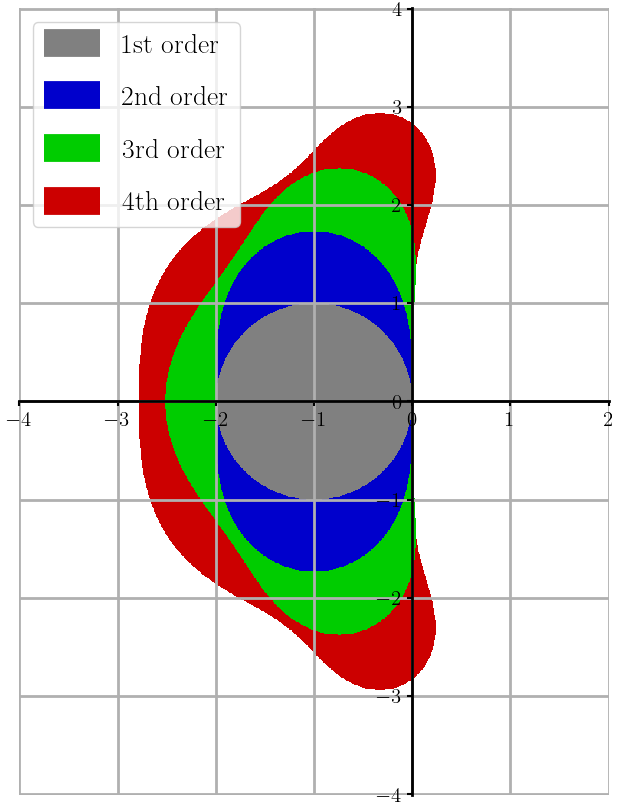
\includegraphics{figures/rk_stab.png}
          \caption{Stability regions (in colour) of the four first-order Runge--Kutta methods.}
          \label{fig:rk_stab}
        \end{figure}

        \paragraph{}
        We can see that Runge--Kutta methods are not A-stable, and they do not have a large stability region.
        Increasing the order of the method does increase the stability region, but not enough for our applications.
        Practically, this imposes the use of small time steps, which is agreeable for unsteady computations but not for our steady ones.
        If one iteration of the method is inexpensive, the total number of iterations needed to reach the steady solution will make the overall computation too costly.


      \subsubsection{Adams--Bashforth methods}

        \paragraph{}
        We could try to use other explicit methods, such as multistep Adams--Bashforth methods.
        The $k$th order Adams--Bashforth method uses the last $k$ computed steps to find the next one.
        One can indeed check that the index $k$ designating the method also corresponds to its order \cite{HairerNorsettWanner1993}.

        \paragraph{}
        The idea is to apply a Lagrange interpolation of the function $\operatorname{G}$ from equation (\ref{eq:init_value_ode}) in the $k$ last computed points, and then replace $\operatorname{G}$ with the interpolation polynomial when integrating from $t_n$ to $t_{n+1}$.
        Contrary to the Runge--Kutta methods, as this method reuses previous information, a single $\operatorname{G}$ evaluation is required at each step.
        Because of that, the cost of one iteration of the Adams--Bashforth method is quite inexpensive.
        The stability analysis for such methods is a bit more complex \cite{HairerNorsettWanner1993, HairerWanner1996}, and so the result obtained numerically is shown on figure \ref{fig:ab_stab} without giving the details.
        The conclusion is even worse than with Runge--Kutta methods, as the stability region decreases as the order increases.
        The Adams--Bashforth methods can reach a high order of accuracy while staying computationally inexpensive, but they drastically lack stability, and that is why they are often not used in computational fluid dynamics computations.
        More generally, an explicit multistep method cannot be A-stable \cite{Dahlquist1963}.

        \begin{figure}
          \centering
          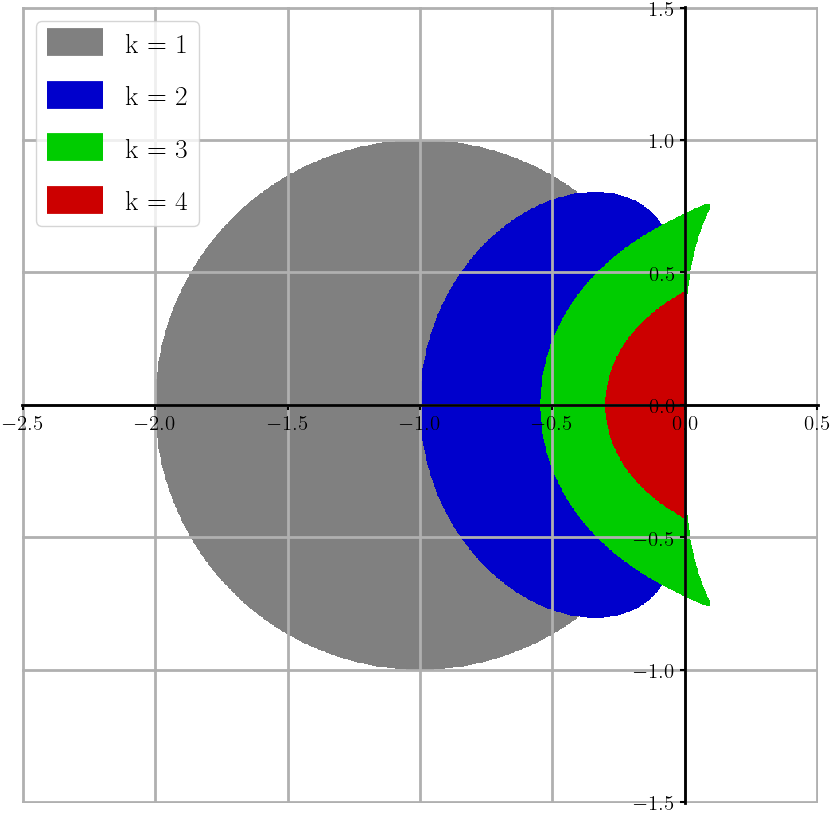
\includegraphics{figures/ab_stab.png}
          \caption{Stability regions (in colour) of the four first Adams--Bashforth methods.}
          \label{fig:ab_stab}
        \end{figure}


    \subsection{Implicit methods}

      \paragraph{}
      We explained in the previous section why explicit time integration methods are not suited for our applications.
      It is then natural to look at implicit methods.
      Contrary to the explicit methods, implicit methods do not give the looked-for solution right away, but as the solution of a specific equation.
      The name is appropriate: the next state is not given explicitly but implicitly.


      \subsubsection{Implicit Euler method}

        \paragraph{}
        The implicit Euler method is the equivalent of the explicit Euler method but on the implicit side.
        It is quite similar, as it consists in integrating equation (\ref{eq:init_value_ode}) assuming the function $\operatorname{G}$ is constant, but this time equal to $\operatorname{G}\left(\Xi_{n+1}\right)$:
        \begin{equation}
          \begin{aligned}
            & \phantom{{} \Leftrightarrow {}} \Xi_{n+1} = \Xi_n + \Delta t \operatorname{G}\left(\Xi_{n+1}\right) \\
            &             \Leftrightarrow     \Xi_{n+1} - \Xi_n - \Delta t \operatorname{G}\left(\Xi_{n+1}\right) = 0
          \end{aligned}
        \end{equation}
        and the next state $\Xi_{n+1}$ is given as the solution of a nonlinear problem, the root of a nonlinear function.

        \paragraph{}
        After checking that this is a first-order method, the stability analysis gives the corresponding function $g\left(z\right) = \left(1 - z\right)^{-1}$, that gives a stability region equal to the whole complex plane minus the closed unity disk centered in 1.
        Therefore this method is A-stable.


      \subsubsection{Implicit Runge--Kutta methods}

        \paragraph{}
        Runge--Kutta methods can also be implicit methods.
        This happens when the quadratures use points that have not already been computed.
        In other words, this corresponds to a full $A$ matrix in the Butcher tableau, where it is strictly lower triangular for explicit Runge--Kutta methods.
        This also means that any step of the Runge--Kutta method may be used in any other step, and therefore one may have to simultaneously solve an implicit system of equations.
        This may lead to awfully expensive methods, and therefore users tend to restrict themselves to some particular methods.

        \paragraph{}
        Despite their cost, implicit Runge--Kutta methods can be appealing.
        The main reason is that they can easily achieve a high order of accuracy.
        For example, the methods based on Gauss--Legendre quadratures achieve an order $2k$ with $k$ steps, and they are all A-stable \cite{Iserles2008}.
        Theoretically, this means that an arbitrarily high order can be achieved while keeping the stability quality with these methods.
        However, users usually stop at the 3-stage 6th order method, as the computational cost tends to be too much for higher order methods.

        \paragraph{}
        When applying the stability analysis to a Runge--Kutta method, one can get the function $g$ using the matrix $A$ and the array $b$:
        \begin{equation}
          g\left(z\right) = 1 + z \transpose{b} \left(\operatorname{Id} - zA\right)^{-1} \transpose{\left(1, \dots, 1\right)} .
        \end{equation}
        We will not try to show the corresponding stability regions as there are too many methods possible.
        Instead, we will review some of the most frequent from the literature.

        \paragraph{Diagonally Implicit Runge--Kutta methods}
        The Diagonally Implicit Runge--Kutta methods \cite{Alexander1977}, or DIRK methods, are Runge--Kutta methods with a lower triangular matrix $A$.
        Then, each step is given as an implicit problem using the already known steps and the next one.
        The difference is that instead of solving a full implicit system, one just needs to solve each implicit step successively.
        This help drastically reduces the cost of the method.
        Furthermore, if all quadrature coefficient $a_{ii}$ are all equals, as each step requires the inversion of the matrix
        \begin{equation}
          \operatorname{Id} - a_{ii} \Delta t \frac{\mathrm{d} \operatorname{G}}{\mathrm{d} \Xi}\left(\Xi_n\right) ,
        \end{equation}
        this can help solving the linear problem.
        This variant is called Singly Diagonally Implicit Runge--Kutta methods (SDIRK) \cite{HairerWanner1996}.

        \paragraph{Rosenbrock methods}
        Rosenbrock methods are also called linearly implicit Runge--Kutta methods \cite{Rosenbrock1963}.
        They start from the recurrence relation of a DIRK method:
        \begin{equation}
          \Xi_{n,i} = \Xi_n + \Delta t \sum_{j = 1}^{i-1} a_{ij} \operatorname{G}\left(\Xi_{n,j}\right) + \Delta t a_{ii} \operatorname{G}\left(\Xi_{n,i}\right)
        \end{equation}
        and then take its image by $\operatorname{G}$.
        Instead of solving this nonlinear equation with a nonlinear solver as the DIRK method would do, they linearize the result:
        \begin{equation}
          \operatorname{G}_{n,i} = \operatorname{G}\left(\Xi_n + \Delta t \sum_{j = 1}^{i-1} a_{ij} \operatorname{G}_{n,j}\right)
          + \Delta t a_{ii} \frac{\mathrm{d} \operatorname{G}}{\mathrm{d} \Xi}\left(\Xi_n + \Delta t \sum_{j = 1}^{i-1} a_{ij} \operatorname{G}_{n,j}\right) \operatorname{G}_{n,i}
        \end{equation}
        by noting $\operatorname{G}_{n,j} = \operatorname{G}\left(\Xi_{n,i}\right)$.
        The recurrence equation for the integration scheme is no longer on the intermediate states but on the intermediate slopes.
        Usually, the Jacobian matrix is kept constant throughout the stages, equal to the Jacobian matrix evaluated in $\Xi_n$.
        Additional parameters $\gamma_{ij}$ are often to add more flexibility to the method \cite{Wanner1977}.
        It gives the Rosenbrock--Wanner method:
        \begin{equation}
          \left\{\begin{aligned}
            \Xi_{n+1} &= \Xi_n + \Delta t \sum_{i = 1}^k b_i \operatorname{G}_{n,i} \\
            \textrm{with}\quad \operatorname{G}_{n,i} &=
              \operatorname{G}\left(\Xi_n + \Delta t \sum_{j = 1}^{i-1} a_{ij} \operatorname{G}_{n,j}\right)
              + \Delta t \frac{\mathrm{d} \operatorname{G}}{\mathrm{d} \Xi}\left(\Xi_n\right) \sum_{j = 1}^{i} \gamma_{ij} \operatorname{G}_{n,j}
          \end{aligned}\right. .
        \end{equation}
        This corresponds to classical Rosenbrock methods when all $\gamma_{ij}$ are null, except for $\gamma_{ii}$ that correspond to the $a_{ii}$.
        However, the distinction is not made very often, and Rosenbrock--Wanner methods are simply called Rosenbrock methods.
        The method is defined by the coefficients $a_{ij, 1\leq j<i\leq k}$, $b_{i, 1\leq i\leq k}$ and $\gamma_{ij, 1\leq j\leq i\leq k}$.
        If the problem is non-autonomous, the method is then:
        \begin{equation}
          \left\{\begin{aligned}
            \Xi_{n+1} &= \Xi_n + \Delta t \sum_{i = 1}^k b_i \operatorname{G}_{n,i} \\
            \textrm{with}\quad \operatorname{G}_{n,i} &=
              \operatorname{G}\left(\Xi_n + \Delta t \sum_{j = 1}^{i-1} a_{ij} \operatorname{G}_{n,j} \ ,\  t_n + c_i \Delta t\right)\\
              &\phantom{= {}} +\Delta t \frac{\partial \operatorname{G}}{\partial \Xi}\left(\Xi_n, t_n\right) \sum_{j = 1}^{i} \gamma_{ij} \operatorname{G}_{n,j} \\
              &\phantom{= {}} +\Delta t \frac{\partial \operatorname{G}}{\partial t}\left(\Xi_n, t_n\right) \sum_{j = 1}^i \gamma_{ij}
          \end{aligned}\right.
        \end{equation}
        with $c_i = \sum_{j = 1}^{i - 1} a_{ij}$ as for other Runge--Kutta methods.
        If one takes all the $\gamma_{ii}$ equals to one another, then the matrix to invert at each step of the Rosenbrock method is the same.
        This can help reduce the cost of the method by doing a single matrix inversion, or by recycling information between Krylov subspace methods \cite{Gaul2014}.
        Overall, even if they can achieve high-order and A-stability, Rosenbrock methods are still computationally expensive.


      \subsubsection{Backward differentiation formula}

        \paragraph{}
        As explicit Runge--Kutta methods are extended to implicit methods, Adams--Bashforth method also have their implicit counterparts.
        The idea is to still compute the Lagrange interpolation of the function $\operatorname{G}$ but with one additional point: the point at the next time step.
        This new method is called the Adams--Moulton method.
        However, the stability region of Adams--Moulton is quite narrow, as they were originally not made for stiff equations \cite{Iserles2008}.
        This is why the Backward Differentiation Formula methods, or BDF methods, were introduced.
        Contrary to Adams--Bashforth and Adams--Moulton methods, they use the Lagrange interpolation of the solution $\Xi$ instead of the interpolation of the function $\operatorname{G}$.
        Then, the time derivative of the solution can be replaced by the time derivative of the interpolating polynomial, and the resulting equality is evaluated at the next time step $t_{n+1}$.
        This gives an implicit equation that is solved to get $\Xi_{n+1}$.
        The name of those methods comes from the fact that if it uses a constant time step between iterations, this equation can be written using the differentiating operator defined by $\nabla^0 \square_i = \square_i$ and $\nabla^{j+1} \square_i = \nabla^j \square_i - \nabla^j \square_{i-1}$:
        \begin{equation}
          \sum_{i=1}^k \frac{1}{i} \nabla^i \Xi_{n+1} = \Delta t \operatorname{G}\left(\Xi_{n+1}\right)
        \end{equation}

        \paragraph{}
        The order of the method is equal to the index of the method, corresponding to the number of previous states needed to compute the next one.
        These methods allow for an arbitrarily high order without increasing the cost, as the implicit equation is not harder to solve as the order increases.
        However, the stability analysis limits the higher order achievable.
        The stability analysis of the BDF methods can be done numerically.
        At this stage, one can note that the first-order BDF method is in fact the implicit Euler method.
        Also, methods of order 7 or higher are unstable, so we can limit our analysis to methods with orders from 1 to 6.
        The corresponding stability regions are satisfying, as can be seen in figure \ref{fig:bdf_stab}.
        Particularly, the first and second methods are A-stable.
        We see when looking at the scales in figure \ref{fig:bdf_stab} that the complement of the stability region grows with the index of the method.
        More generally, there are no A-stable multistep methods with orders higher than 2 \cite{Dahlquist1963, HairerWanner1996}.

        \begin{figure}
          \centering
          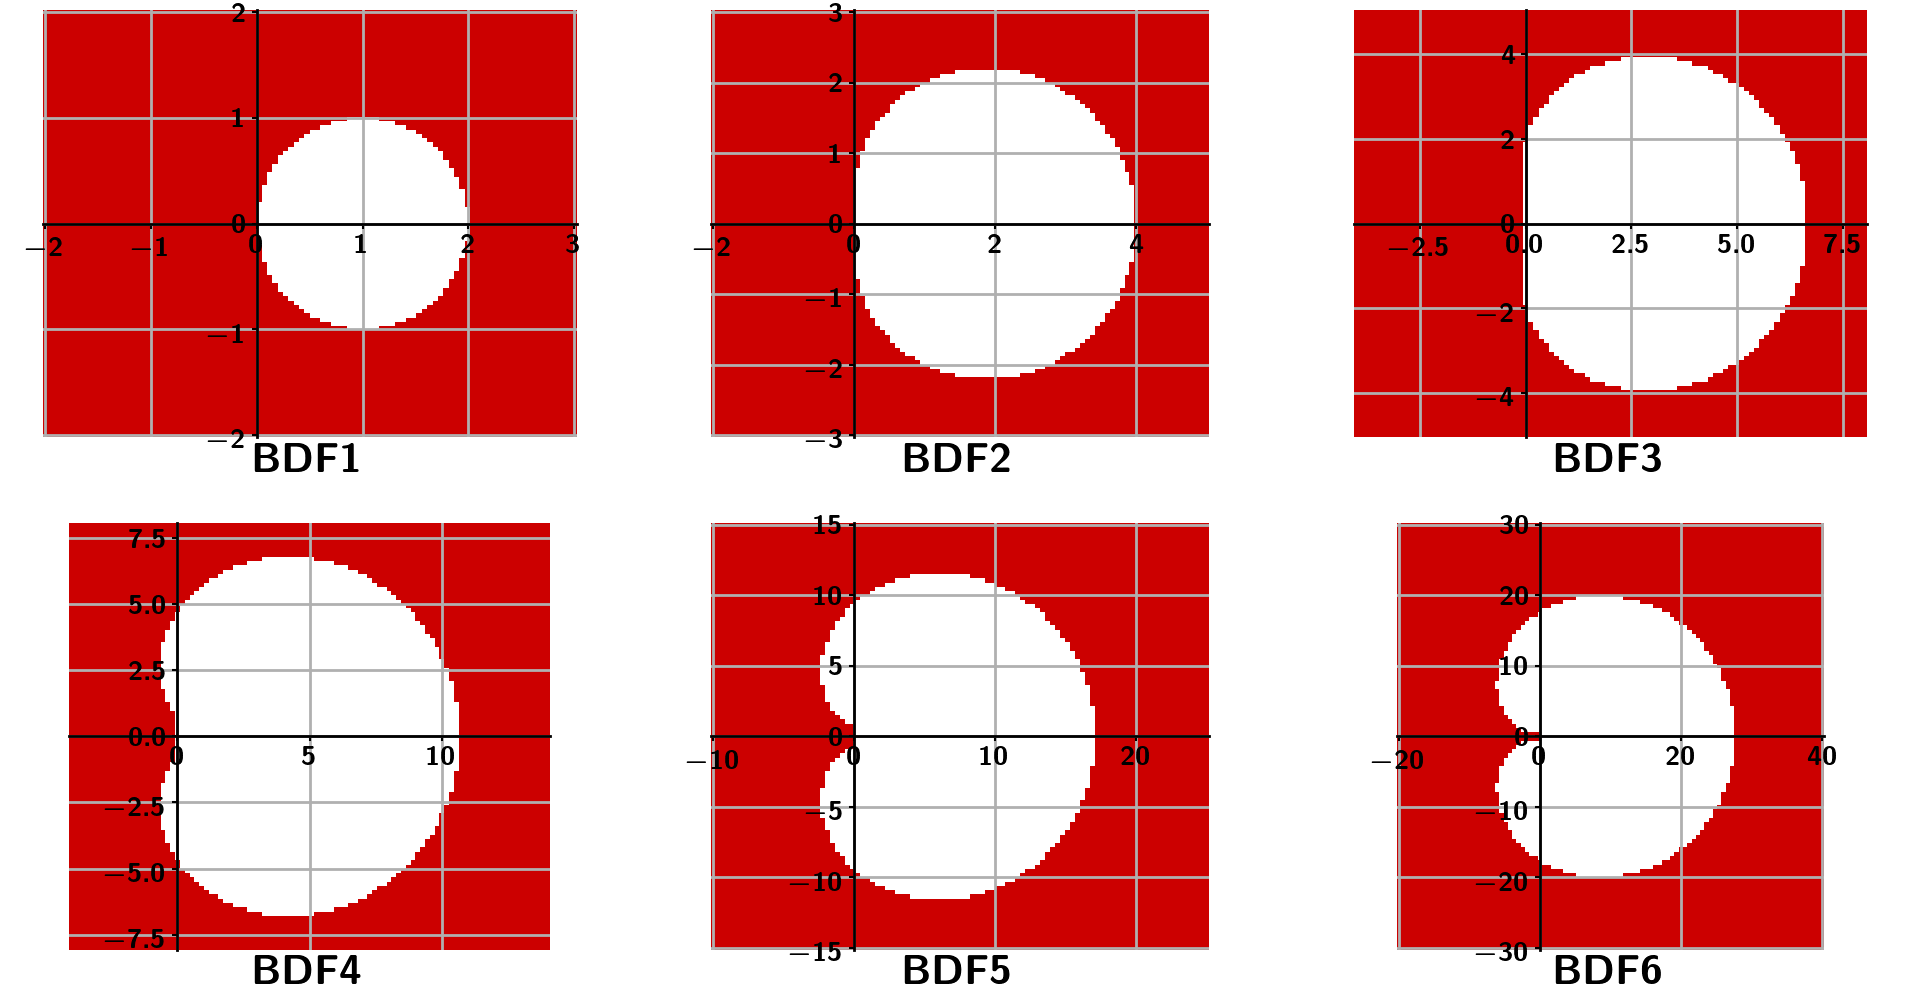
\includegraphics{figures/bdf_stab.png}
          \caption{Stability regions (in colour) of the BDF methods. Zoom is not constant between plots.}
          \label{fig:bdf_stab}
        \end{figure}

      \paragraph{}
      This introduction to the classic time integration methods helps us to decide what to do for our solver.
      As we said earlier, we want to solve an ordinary differential equation in order to recover the steady solution, reached after a long time.
      Then, explicit methods that constrain the time step are not well fitted.
      Even if they cost more, algorithmically speaking, implicit methods are indeed the best choice for stiff equations.
      It is often better to do a single expensive iteration over a large time step with an implicit method than make a lot of inexpensive iterations over small time steps with an explicit method.
      This is finally why we will continue working with the A-stable implicit Euler method.
      This method is already used in our solver as the base implicit method, for the same reasons we want to use it.
      Furthermore, it is at the base of all other implicit methods, as they can be seen as small variations of the implicit Euler methods.
      Choosing it is also smart as updating it into another implicit time integration method will not require too much work.


  \section{Implicit methods framework}

    \subsection{Methodology of the implicit time integration}

      \paragraph{}
      As we explained in the previous section, implicit time integration methods give the next state as the solution of a nonlinear equation or a system of nonlinear equations.
      If we want to use implicit methods, we then need to be able to solve a nonlinear problem.
      We will continue our discussion using the implicit Euler method, but everything can easily be adapted for any other implicit method.
      For Diagonally Implicit Runge--Kutta methods, we apply the nonlinear solver successively for each step.
      For BDF methods, we apply the nonlinear solver on a slightly different equation.


      \subsubsection{From a nonlinear problem \dots}

      	\paragraph{}
      	Newton's method can be used to solve a nonlinear problem of the form:
      	\begin{equation}
      		\tilde{f}\left(\Xi_{n+1}\right) = 0 .
      	\end{equation}
        Equivalently, as it works for a single $n$ at a time, this equation can be expressed in terms of the increment $x = \Xi_{n+1} - \Xi_n$ without writing the subscript:
        \begin{equation}\label{eq:nonlinear}
      		f\left(x\right) = 0 .
      	\end{equation}
        Newton's method starts from an initial guess $x_0$.
        This initial guess is often equal to zero, as it is equivalent to taking $\Xi_n$ as an initial guess for $\Xi_{n+1}$.
        The method will then iterate to approximate the solution of equation (\ref{eq:nonlinear}).

        \paragraph{}
        At each step of Newton's method, the problem is linearised in the current estimation $x_i$ and the new equation is evaluated at the next iteration $x_{i+1}$:
        \begin{equation}\label{eq:nonlinear_linearised}
          f\left(x_{i+1}\right) \approx f\left(x_i\right) + f'\left(x_i\right) \left( x_{i+1} - x_i \right) = 0
        \end{equation}
        This gives a linear problem in which $x_{i+1}$ is the solution.


      \subsubsection{\dots to a linear one}

        \paragraph{}
        Equation (\ref{eq:nonlinear_linearised}) can be rewriten into the classic linear problem:
        \begin{equation}\label{eq:linear}
          Ax = b
        \end{equation}
        where $A = f'\left(x_i\right)$, $b = -f\left(x_i\right)$ and $x = \left( x_{i+1} - x_i \right)$.
        The $x$ notation is reused as it is often used in the literature to name the unknown in linear problems.
        Such linear problems are found during the iterations of Newton's method, but each is solved for a given iteration number so there are no ambiguity from this notation.
        A lot of methods were conceived to solve such linear problems, and we will explain later how to handle them.


      \paragraph{}
      To sum up, we started from the partial differential equation (\ref{eq:pde}) arising from the physical model.
      With a spatial discretisation method, and after choosing an initial value, this transforms into an ordinary differential equation (\ref{eq:init_value_ode}).
      For stability reasons, we decided to use implicit time integration methods.
      Iteratively, such methods are going to produce one or several nonlinear problems in the form of equation (\ref{eq:nonlinear}).
      Newton's method used to solve such problems is going to produce a succession of linear problems in the form of equation (\ref{eq:linear}).
      This complicated sequence of operations describes the time integration procedure used in our solver to find the solution to steady problems.
      It is schematised in figure \ref{fig:steady_solve}, where the blue circles correspond to the problems being solved, while green circles correspond to the methods used to solve them.
      In this thesis, we are interested in the non-greyed parts.\GP{J'ai pas compris ce qui est non grisé... Aurais-je un souci d'affichage ?}

      \begin{figure}
        \centering
        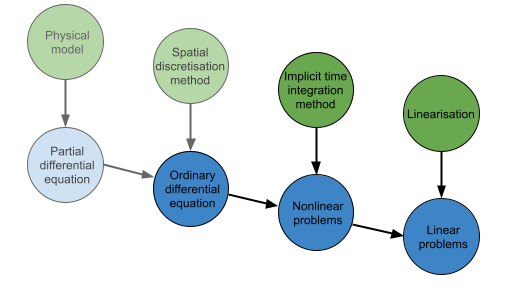
\includegraphics{figures/steady_solve.png}
        \caption{Procedure used to find the solution of steady problems.}
        \label{fig:steady_solve}
      \end{figure}


    \subsection{Nonlinear solver}

      \paragraph{}
      As we said, we solve the nonlinear problem with Newton's method.
      What was done in our solver was in fact a single step of Newton's method, which means a single linearization of the nonlinear problem.
      Since we could benefit from an actual Newton's method, it was implemented.
      Contrary to the single linearisation that was done before, several linear problems need to be solved during one single time step, so several Jacobian matrices are needed.

      \paragraph{}
      The issue when using Newton's method is that it should be accompanied by a Line Search algorithm to determine the step size $\alpha$ so that the next iterate of the method is:
      \begin{equation}
        x_{i+1} = x_i - \alpha f'\left(x_i\right)^{-1} f\left(x_i\right) .
      \end{equation}
      During this thesis, we did some work towards using a complete Newton's method, but we did not have time to develop a Line Search algorithm, so we ended up using the standard method from our solver: a single linearization of the nonlinear problem.


    \subsection{Linear solver}

      \paragraph{}
      We want to be able to solve efficiently linear systems like (\ref{eq:linear}).
      We additionally assume that $A$ is an invertible matrix.
      Let us note the size of the linear system $N$.
      This size is quite large in our typical applications, but the linear system is sparse.
      This means that the coefficients of the matrix $A$ are mostly zeros.
      This is because a coefficient in the matrix $A$ corresponds to a link between two degrees of freedom.
      For the considered spatial discretisation methods, a cell only depends on a small number of neighbouring cells, and therefore a degree of freedom is not linked with most of the others.
      In practice, the stencil is generally reduced to the current cell and those that share a face with the current cell.
      This transcribes into lots of zeros in the matrix, and therefore its sparsity.
      Such sparse matrices can be seen in figure \ref{fig:sparse}.
      Using the sparsity of the matrix is essential, as it would not be possible to store it as a dense matrix in the memory of a computer.
      Instead, some clever formats are used, such as the Compressed Sparse Row format \cite{Saad2003}.
      Some operations such as matrix-vector products are more efficiently done using such formats.

  		\begin{figure}
  			\centering
  			\begin{subfigure}[t]{0.3\textwidth}
  				\centering
  				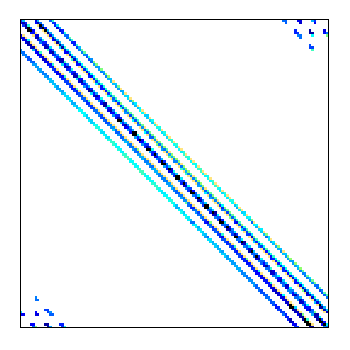
\includegraphics[width=\textwidth]{figures/GT01R.png}
          \caption{GT01R: 2D inviscid flow in the inter-blade channel of a linear cascade turbine.}
  				\label{fig:sparse.GT01R}
  			\end{subfigure}
  			\hfill
  			\begin{subfigure}[t]{0.3\textwidth}
  				\centering
  				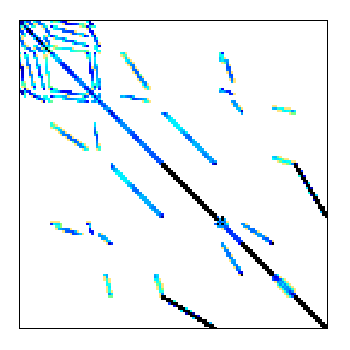
\includegraphics[width=\textwidth]{figures/HV15R.png}
  				\caption{HV15R: 3D RANS simulation of an engine fan.}
  				\label{fig:sparse.HV15R}
  			\end{subfigure}
  			\hfill
  			\begin{subfigure}[t]{0.3\textwidth}
  				\centering
  				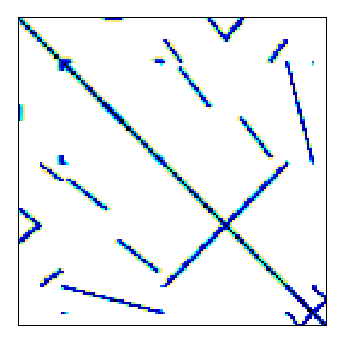
\includegraphics[width=\textwidth]{figures/RM07R.png}
  				\caption{RM07R: 3D viscous flow in a jet engine compressor.}
  				\label{fig:sparse.RM07R}
  			\end{subfigure}
  			\caption{Matrices from various CFD simulations \cite{PacullAubertBuisson2011} using a Finite Volume method. Coloured points correspond to nonzero values.}
  			\label{fig:sparse}
  		\end{figure}

      \paragraph{}
      Many methods exist to solve linear problems.
      Some are even taught in school, such as the Gaussian elimination.
      Such methods are called direct methods, as they first do some work and then find directly the exact solution to the problem.
      But for problems with huge sizes such as the ones encountered in computational fluid dynamics, the amount of work is too much to be computed with today's means.
      It would take too much time as well as too much memory.
      Instead, one can use iterative methods.
      An iterative method starts from an initial guess $x_0$ and produces as it iterates a supposedly better estimation of the solution $x_n$.
      The subscript $n$ has nothing to do with the subscript used to identify the iterates of the time integration method: this hapens at a given fixed time step.
      We can then decide when to stop the method, whether the solution estimate is good enough or the resolution is taking too much time.
      Iterative methods are the most well-fitted to solve large sparse linear problems, and they are the preferred solution in computational fluid dynamics.

      \paragraph{}
      Among the iterative methods are what could be called the "classic" methods, or relaxation.
      They are the Jacobi, Gauss--Seidel or Successive Over Relaxation methods.
      They decompose the matrix into $A = M - N$ with $M$ a matrix easily invertible.
      The choice of $M$ depends on the method.
      Then, starting from a given $x_0$, each step computes $x_{n+1} = M^{-1} \left( N x_n + b \right)$.
      Those methods are often deemed not efficient enough for computational fluid dynamics applications.
      They are often used, however, as preconditioning methods, as we will see later.

      \paragraph{}
      Another class of iterative methods is becoming the standard for computational fluid dynamics: the Krylov subspace methods.
      A Krylov subspace method projects the linear problem (\ref{eq:linear}) on a smaller linear subspace called Krylov subspace.
      The obtained smaller system is then solved, much more easily.
      The cleverness resides in the fact that those Krylov subspaces are nested, and each iteration reuses the information obtained in the previous ones.

      \paragraph{}
      In the following, we note at iteration $n$ the residual $r_n = b - A x_n$.
      Practically, we keep $n \ll N$ so that the cost of the method stays reasonable, but this does not change the following.
      The corresponding Krylov subspaces are defined as:
  		\begin{equation}
  			\krylov[A, r_0]{n} = \operatorname{Vect}\left( r_0, A r_0, \dots, A^{n-1} r_0 \right) .
  		\end{equation}
      Then, the next iterate in $\krylov{n}$ must satisfy a Petrov--Galerkin condition \cite{SimonciniSzyld2007}:
  		\begin{equation}
  			x_n \in x_0 + \krylov[A, r_0]{n} \quad \textrm{such as} \quad r_n \perp \mathcal{L}_n
  		\end{equation}
      where $\mathcal{L}_n$ is a linear subspace with dimension $n$.
      For example, $\mathcal{L}_n = \krylov{n}$ corresponds to a Galerkin condition, and $\mathcal{L}_n = A \krylov{n}$ is a minimum residual condition.

      \paragraph{}
      To construct the growing Krylov subspace, one can use the Arnoldi iteration \cite{TrefethenBau1997}.
      As a result, the matrix $A$ is only used through matrix-vector products.
      Indeed, Krylov subspace methods do not require the matrix $A$ to solve the linear system (\ref{eq:linear}), just to know how to compute matrix-vector products.
      We will use this property later on.

      \paragraph{}
      There are many Krylov subspace methods that can solve a linear problem, characterised by the choice of $\mathcal{L}_n$.
      The minimal residual condition gives the Generalized Minimal Residual method or GMRES \cite{SaadSchultz1986}, vastly used in computational fluid dynamics \cite{FrancoCamierAndrejEtAl2020} and other fields of numerical simulations \cite{ErnstGander2012, Mercier2015}.
      Its main advantage is that even if its iterations may be slightly more expensive than other methods such as the Bi-CGSTAB method \cite{Vorst1992, TrefethenBau1997}, the residual norm is minimised and the error is then decreasing as the method iterates.
      This allows for some control of the residual norm.
      With the Bi-CGSTAB method for example, also available in our solver, the residual norms do not have to be decreasing, which can lead to chaotic convergence.
      The GMRES method already exists in our solver and is often used.
      Because it is discussed a lot in the literature, many variants and enhancements were developed \cite{CoulaudGiraudRametEtAl2013, Vasseur2016, JolivetTournier2016}.
      For those reasons, we decided to keep the GMRES method as the base of our linear solver.

      \paragraph{}
      The convergence of Krylov subspace methods, and more generally of iterative methods, depends on the linear system matrix.
      It is common knowledge that the convergence is linked to the condition number of the matrix \cite{Nevanlinna1994}.
      The condition number of an invertible matrix $A$ is defined as:
      \begin{equation}
        \kappa\left( A \right) = \norm{A} \norm{A^{-1}}
      \end{equation}
      and so it depends on the chosen norm.
      A problem is said to be well-conditioned when $\kappa = O\left(1\right)$, and ill-conditioned when $\kappa \gg 1$.
      For the Euclidean norm $\norm[2]{\cdot}$,
  		\begin{equation}\label{eq:conditioning}
  			\kappa\left( A \right) = \frac{\sigma_{\max}}{\sigma_{\min}}
  		\end{equation}
      where $\sigma_{\min}$ and $\sigma_{\max}$ are the smallest and largest singular values of the matrix $A$.
      As a reminder, the singular values of $A$ are the eigenvalues of $A^* A$ where $A^*$ notes the conjugate transpose of $A$.
      The relation (\ref{eq:conditioning}) is often simplified as
      \begin{equation}
        \kappa\left( A \right) = \frac{\left|\lambda_{\max}\right|}{\left|\lambda_{\min}\right|}
      \end{equation}
      with $\lambda_{\min}$ and $\lambda_{\max}$ the eigenvalue of $A$ with the smallest and largest modulus.
      If this helps picture what the condition number stands for, this is only true for normal matrices: matrices that commute with their conjugate transpose.
      However, the matrices we face in our field have no reasons to be normal matrices.
      An intriguing result is found in \cite{GreenbaumPtakStrakos1996}.
      For a given decreasing convergence curve and a given spectrum, it is possible to construct a linear problem such as the convergence of GMRES follows the given curve and the matrix has the given spectrum.
      In other words, there are ill-conditioned matrices for which GMRES converges quickly and well-conditioned matrices for which GMRES will be slow.
      In particular, one can find a matrix with the best condition number possible, meaning 1, on which GMRES will make no progress until the last iteration.
      This is because of the nonnormality of the matrix \cite{GreenbaumStrakos1994, GreenbaumPtakStrakos1996}.
      To handle it in the analysis of the convergence, one must not look at the spectrum but the pseudospectrum \cite{Trefethen1991, Trefethen1999}.
      This analysis is quite complex and is mostly done in an analytical context, not an industrial one.
      Using Krylov subspace methods with nonnormal matrices and the study of their convergence is no simple task \cite{LiesenTichy2004, Huhtanen2005}.
      As the matrices we encounter in our computational fluid dynamics problems are arbitrary, meaning mostly nonnormal, we decided not to study finely the spectrum of the operator.

      \paragraph{}
      Even if we will not look deeply into the spectrum of the matrix, we still help the linear solver with preconditioning.
      Preconditioning consists in multiplying the equation (\ref{eq:linear}) with a preconditioning operator $P$ to the left for left preconditioning:
      \begin{equation}
        PAx = Pb
      \end{equation}
      and to the right for right preconditioning:
      \begin{equation}
        \left\{\begin{aligned} APx' &= b \\	Px' &= x \end{aligned}\right. .
      \end{equation}
      The idea is to transform $A$ into a matrix that is more easily invertible.
      The matrix to invert is now $PA$ for left preconditioning and $AP$ for right preconditioning.
      If the preconditioning operator is close to $A^{-1}$ and is cheap to compute, this new matrix is close to $\operatorname{Id}$ and so is easily invertible.
      If $P$ is too close to $A^{-1}$, computing the preconditioning will be as expensive as solving the original linear problem.
      If $P$ is too easy to compute, meaning close to $\operatorname{Id}$, the preconditioning will be useless.
      Choosing a preconditioner means making a compromise between those two extrema.

      \paragraph{}
      Just as Krylov subspace methods only need to compute matrix-vector products, and not to know the matrix, we do not need to know the preconditioning matrix, but only to know how to apply it on any given vector.

      \paragraph{}
       To better understand how preconditioning works, let us take an example, inspired by example 35.2 of \cite{TrefethenBau1997}.
       We take a square matrix of size 200 by 200, which is the sum of a diagonal part and a random perturbations part:
       \begin{equation}
         \begin{aligned}
           A &= A_{diag} + \frac{1}{2\sqrt{N}}A_{rand} \\
           \textrm{where}\quad A_{diag, k} &= 2\sin\left( \frac{2 k \pi}{N - 1} \right) - 1 + i \cos\left( \frac{2 k \pi}{N - 1} \right) \\
           \textrm{and}\quad A_{rand} &\hookrightarrow \mathcal{N}\left(0, 1\right) .
         \end{aligned}
       \end{equation}
       The vector $b$ is a vector of ones.
       The spectrum of $A$ is displayed in figure \ref{fig:preconditioning} in blue.
       It is spread out around the origin.
       When we apply the Jacobi preconditioning, meaning the preconditioning matrix is the invert of the diagonal part, the spectrum is gathered around 1.
       This helps a lot GMRES, as can be seen in figure \ref{fig:preconditioning}: it struggles to reduce the residual norm on the standard problem but does it easily on the preconditioned problem.
       This is only a dummy example, but it helps visualise the importance of preconditioning.

   		\begin{figure}
   			\centering
   			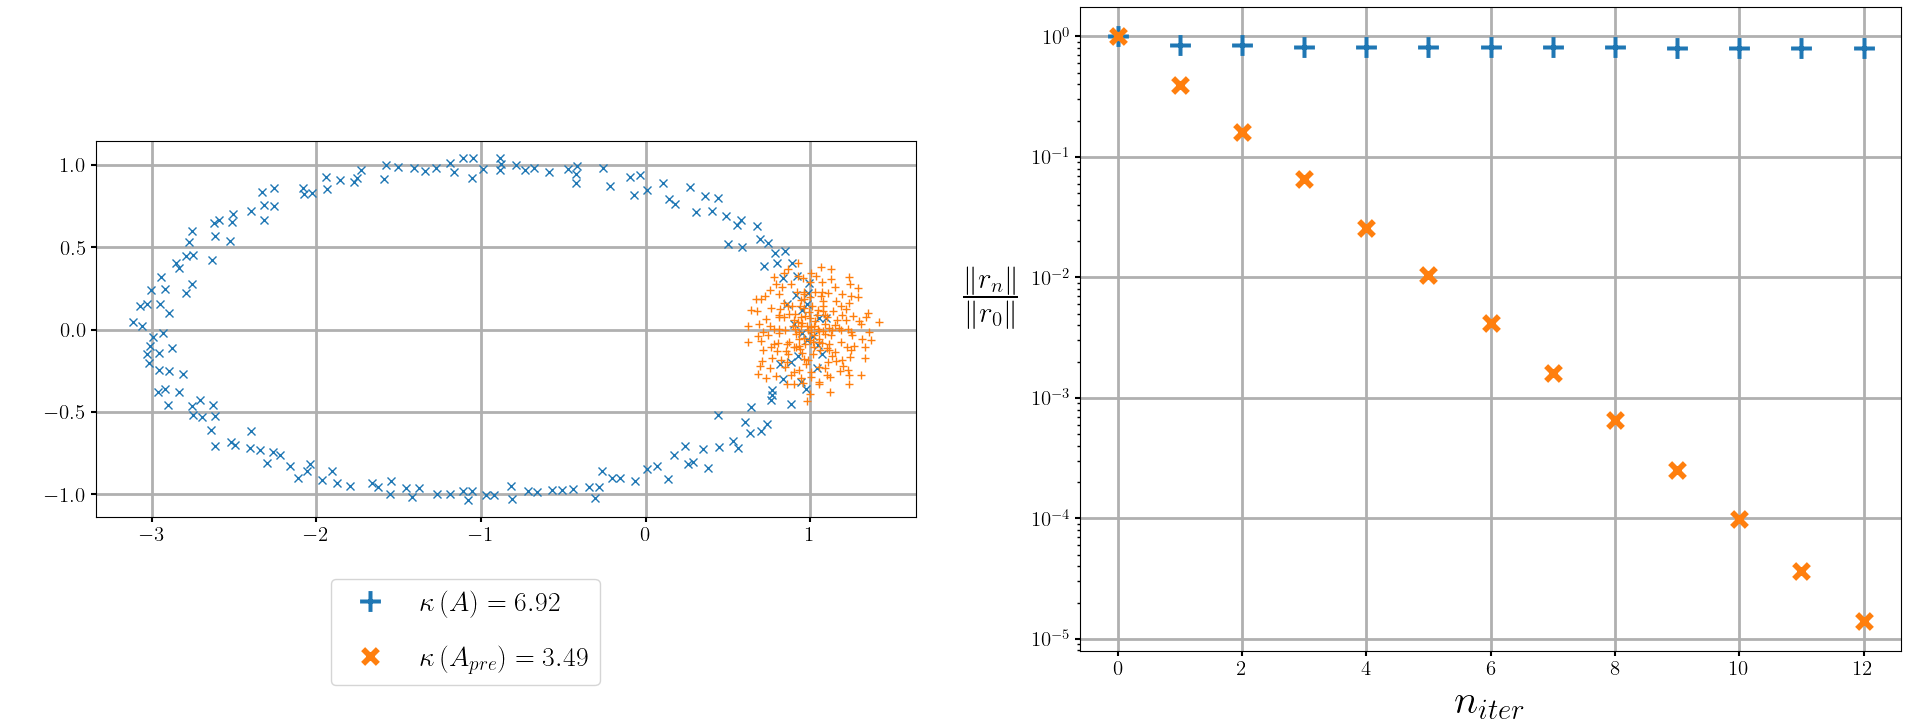
\includegraphics{figures/preconditioning.png}
   			\caption{Spectrum of $A$ in blue and $A_{pre} = AD^{-1}$ in orange (left). GMRES convergence for those matrices (right).}
   			\label{fig:preconditioning}
   		\end{figure}

      \paragraph{}
      We need to use preconditioners when solving the linear system (\ref{eq:linear}) with GMRES.
      One of the less sophisticated preconditioners is the Jacobi one.
      It is the one used in the example above: the preconditioning matrix is the invert of the diagonal part of $A$.
      Its advantage resides in its simplicity.
      It is inexpensive and easily scalable.
      On the other hand, it lacks efficiency, and that is why many preconditioners were developed in the literature.
      A slight variation consists in taking the diagonal blocs instead of the diagonal elements.
      This makes sense for our matrices, as they can be divided into blocs, each block corresponding to the degrees of freedom in a cell.
      The resulting preconditioner, called Block Jacobi, already exists in our solver and is often used as the standard preconditioner.

      \paragraph{}
      Others preconditioners exist in our solver.
      One consists in using the invert of the cell volumes as a diagonal matrix: the preconditioning matrix is a diagonal matrix, where each diagonal element is the inverse of the corresponding mesh cell volume.
      This was originally conceived to preserve the conservative properties through the GMRES solve.
      Indeed, as GMRES produces an approximation of the linear problem solution, the overall scheme may not be conservative.
      This preconditioner makes sure it is.
      More explanations on this statement can be found in appendix \ref{appendix:conservative_preconditioning}.
      As it is even simpler than the Jacobi preconditioner, it shows poor performance.
      Some work was done towards Polynomial preconditioning: the preconditioning matrix $P$ is equal to the partial Neumann series of $\operatorname{Id} - A$, as it approximates $A^{-1}$ \cite{DuboisGreenbaumRodrigue1979}.
      Its major drawback is its computational cost, as it requires multiple matrix-vector products.
      For this reason, we decided not to look into it.

      \paragraph{}
      We were at first interested in some other preconditioners found in the literature, such as the Incomplete LU preconditioner.
      When taking the LU factorisation of the sparse matrix $A$, the triangular matrices $L$ and $U$ lose the sparsity pattern of $A$.
      This is troublesome as it is not possible to store dense matrices of the size of $A$.
      The Incomplete LU preconditioner, characterised by its index $k$, computes only the coefficients of the triangular factors that belong to the sparsity pattern of $A^{k+1}$.
      This way, the factorisation is incomplete in the sense that it does not recreate $A$, but it is still sparse and can be used as a preconditioner.
      The Incomplete LU factorisation is often used in computational fluid dynamics \cite{LiuZhangZhongEtAl2015, AhrabiMavriplis2020}, but it was not a good fit for our solver, due to the difficulty in developing the method in an industrial-size solver, and because it relies directly on the matrix.
      Indeed, the matrix available to us is not precise, as we will explain later, so using it as a preconditioner may not work as well as expected.

      \paragraph{}
      As the preconditioning matrix $P$ is not explicitely needed, and its effect should be near $A^{-1}$, one could take as a preconditioning procedure another Krylov subspace method: to apply the preconditioning to any vector $v$ would mean solving $Ax = v$ with a Krylov subspace method.
      However, applying a Krylov subspace method is not a linear operator.
      To handle this case, the GMRES algorithm must be modified into the Flexible Generalized minimal residual method, or FGMRES \cite{Saad1993, SimonciniSzyld2002}.
      GMRES can be preconditioned with an inner GMRES, and as GMRES was already written in our solver this idea was simple to implement.
      This preconditioning does not need more information on the matrix $A$ than the outer GMRES does: in particular it does not require knowing the matrix coefficients.
      This is interesting for some reasons that are discussed later.
      Finally, this method interests many scientists \cite{CoulaudGiraudRametEtAl2013, Vasseur2016} and has shown promising results in numerical simulation \cite{Pinel2010}.
      For all those reasons, we decided to add this method to our solver.

      \paragraph{}
      The GMRES method is often used with restarting: instead of keeping on iterating the method, one could stop it and start again.
      This is the Restarted GMRES method.
      The cost of one iteration increases as the method iterates.
      Restarting allows for some control of the Krylov subspace dimension, and therefore on computational cost and memory usage.
      The issue with restarting is that it can be harmful to the convergence.
      When the Krylov subspace generated on the restart is too close to the previously generated Krylov subspace, the residual norm may stagnate \cite{Simoncini1999}.
      A solution to this problem would be to reuse information between restarts.
      This is done with the Loose GMRES method \cite{BakerJessupManteuffel2005} or with Augmentation or Deflation techniques  \cite{ChapmanSaad1997, Morgan2002, RamosKehlNabben2020}.
      Augmentation and Deflation give in fact equivalent results \cite{CoulaudGiraudRametEtAl2013}.
      Their idea is to recycle the spectral information acquired at the end of the cycle onto the next cycle.
      Recycling spectral information could even be done throughout multiple linear solve, during a nonlinear solve for example \cite{Gaul2014}.
      Those techniques look promising but we did not have time to try them in our solver, as we focused on other points.


    \subsection{Evaluating the Jacobian matrices}

      \paragraph{}
      If we can solve precisely linear problems, but the problem is not the one the nonlinear solver wants, it may hurt the nonlinear solver convergence.
      We then need to be able to get the right linear problem from the nonlinear one.
      At this point, we know how to evaluate the function $f$ from equation (\ref{eq:nonlinear}), which is often expressed as a linear combination of previous states and $\operatorname{G}$ evaluations, where $\operatorname{G}$ is the function introduced in equation (\ref{eq:init_value_ode}), the function from the starting ordinary differential equation.
      On the other hand, computing its derivative with regard to $x$ is a different story.
      As this derivative is the matrix used when solving the linear problem, it is crucial to have a good representation of it.
      This derivative $f'\left(x\right)$ uses the Jacobian matrix of the function $\operatorname{G}$.
      As the function $\operatorname{G}$ comes from the spatial discretisation method applied to the original partial differential equations (\ref{eq:pde}), it is quite complex to evaluate this Jacobian.
      The underlying algorithm is hard to fully understand and write, and the numerical evaluation is usually expensive.
      Furthermore, our software keeps evolving, and models are constantly added and modified.
      It would require constant work to maintain the Jacobian matrix computation.
      Computing by hand the exact Jacobian matrix would amount to too much work in our industrial software.
      We must use other alternatives to get the Jacobian matrix we need for Newton's method.

      \paragraph{}
      An idea would be to use \emph{Automatic Differentiation} \cite{Griewank2000}.
      This means to give the source code of the $\operatorname{G}$ function to some software \cite{HascoeetPascual2012}, which gives in return a way to compute its Jacobian matrix.
      One advantage of this method is that the cost of derivating the function is done only once, at software compilation.
      After that, computing the Jacobian matrix amount to calling a function.
      Another advantage is that the given Jacobian is supposedly exact, contrary to some alternatives we will discuss later.
      For those reasons, Automatic Differentiation is today being used in actual computational fluid dynamics software \cite{BilanceriBeuxElmahiEtAl2011, KenwayMaderHeEtAl2019}.
      In our software, using Automatic Differentiation did seem too hard and therefore we looked at other methods instead.

      \paragraph{}
      A possible idea is to use an approximation of the Jacobian matrix that is inexpensive to compute.
      We said that the function $\operatorname{G}$ comes from the second-order or higher-order Finite Volume method used as the spatial discretisation method.
      One can then take the function $\operatorname{G}_1$ given by the first-order corresponding method, and use its Jacobian matrix instead.
      Indeed, computing $\operatorname{G}_1$ is inexpensive in comparison to $\operatorname{G}$, and the same goes for the corresponding Jacobian matrices.
      Going further, one could also approximate the Jacobian matrix of $\operatorname{G}_1$: when $\operatorname{G}$ uses some complex models such as turbulence models, it is often decided to not include those models' contributions to the Jacobian matrix, for complexity and stability reasons \cite{ContentOuttierCinnella2013}.
      This is what is done originally in our in-house solver: using a cheap low-order approximation of the Jacobian matrix.

      \paragraph{}
      When we decided to use Krylov subspace methods as our linear solver, we highlighted the fact that they only need to know how to compute matrix-vector products.
      Using this, and the fact that the matrix is a Jacobian matrix, one could approximate the matrix-vector product of $f'\left(x\right)$ with a vector $v$ by:
      \begin{equation}\label{eq:matrix_free}
        f'\left(x\right) v \approx \frac{f\left(x + \varepsilon v\right) - f\left(x\right)}{\varepsilon}
      \end{equation}
      with a scalar parameter $\varepsilon$ discussed below.
      This is the finite difference approximation of the Jacobian matrix-vector product.
      A quick analysis shows that the error on this approximation is $o\left(\varepsilon\right)$.
      Usually, the value of $f\left(x\right)$ is previously computed, so one evaluation of $f$ is required for one matrix-vector product.
      One could also use the centered finite difference approximation:
      \begin{equation}
        f'\left(x\right) v \approx \frac{f\left(x + \varepsilon v\right) - f\left(x - \varepsilon v\right)}{2\varepsilon}
      \end{equation}
      that gives a smaller error of $o\left(\varepsilon^2\right)$, but it requires two $f$ evaluations, so it is twice as expensive as the first-order approximation.
      Therefore, we will use the first-order approximation.

      \paragraph{}
      Using this approximation, it is possible to recover the full Jacobian matrix.
      If the approximation (\ref{eq:matrix_free}) is applied to each vector of the canonical basis as the vector $v$, one can gather each column of the Jacobian matrix.
      This gives what is often called the finite difference Jacobian matrix.
      Instead of computing a matrix-vector product for each direction, a technique consists of computing independent directions beforehand to get a colouring of the matrix: two directions are of the same colour if they are independent through the matrix.
      Then, a smaller number of matrix-vector product approximations are required: as many as there are colours.
      This is often called the finite difference Jacobian matrix with colouring \cite{GebremedhinMannePothen2005}.
      Those techniques are still not well fitted for our solver.
      As we work with large dimensions, computing the Jacobian matrix takes time.
      Furthermore, we explained that we do not need to know explicitly the matrix.
      That is why we will use the approximation (\ref{eq:matrix_free}) each time we need a matrix-vector product instead of computing the Jacobian matrix first.

      \paragraph{}
      We still have not talked about the parameter $\varepsilon$ introduced in equation (\ref{eq:matrix_free}).
      As it represents the size of the step made to approximate a derivative, it should be small.
      But taking it too small leads to roundoff errors so it must be chosen carefully \cite{KnollKeyes2004}.
      We decided to look at some strategies in the choice of $\varepsilon$, and this work will be presented in a later part.

      \paragraph{}
      Now the choices we made for our nonlinear and linear solve strategies are starting to make sense.
      Working with different Jacobian matrices is not an issue, as they are not computed.
      The Krylov subspace method GMRES does not need the Jacobian matrix, only to compute matrix-vector products, contrary to other iterative methods such as the Gauss--Seidel method.
      The flexible preconditioning also does not need the Jacobian matrix for the same reason, contrary to other types of preconditioners such as ILU preconditioners.

      \paragraph{}
      Overall, using Newton's method to solve the nonlinear problem and a Krylov subspace method to solve the linear problem while using a matrix-free method is known as the Jacobian-Free Newton--Krylov method, or JFNK.
      This methods and its variants are as of today still discussed \cite{AnWenFeng2011, Turpault2003} and used on actual computational fluid dynamics solvers \cite{LiuZhangZhongEtAl2015, FrancoCamierAndrejEtAl2020}.
      We are interested in the JFNK method as we hope it will give a better representation of the Jacobian matrix than the low-order one already in use in our solver.
      We hope that a better Jacobian matrix will lead to a better convergence, in particular when some models are ignored in the classic Jacobian matrix, such as turbulence models.

      \paragraph{}
      Furthermore, CEDRE works with multiple distinct solvers.
      When a computation uses multiple solvers, two, for example, the function $f$ from equation (\ref{eq:nonlinear}) is in fact $\left(f_1, f_2\right)$ and $x$ is $\left(x_1, x_2\right)$.
      The Jacobian matrix is then:
      \begingroup
      \renewcommand*{\arraystretch}{1.5}
      \begin{equation}
        f'\left(x\right) = \begin{pmatrix} \frac{\partial f_1}{\partial x_1} & \frac{\partial f_1}{\partial x_2} \\ \frac{\partial f_2}{\partial x_1} & \frac{\partial f_2}{\partial x_2} \end{pmatrix} .
      \end{equation}
      \endgroup
      The cross-term Jacobian matrices, $\frac{\partial f_i}{\partial x_j}$ with $i \ne j$, are usually hard to compute, both analytically and computationally, and are the main obstacle to a fully implicit solver.
      Instead, in CEDRE, each solver iterates independently to the others, with some exchanges between iterations.
      Using the matrix-free approximation and the JFNK method, those cross-solver terms are taken into account.
      This choice is then perfectly aligned with the direction our solver is aiming: towards a better implicit cross-solver mechanism.

      \paragraph{}
      Some specific situations are known to be troublesome for the JFNK method, such as shocks, reaction fronts of discontinuities arising from high order advection schemes \cite{KnollKeyes2004}.
      Unfortunately those features are precisely at the center of our solver.
      We are hopping that the difficulties of the method will be overbalanced by its advantages: getting a better convergence, allowing a fully coupled implicit solve and allowing implicit integration method for new models.
      It means that we do not expect the method to enhance the robustness of the solver, but we hope that because it uses a better Jacobian matrix than the one already in use it will help the convergence.
      And once again, the second advantage is that the matrix-free method would allow us to do coupled implicit time integration.
      We will come back on the third advantage later in the applications part.


    \paragraph{}
    In this section, we described how an implicit method operates: the method itself produces one or several nonlinear problems at each time step.
    Those problems are solved with a nonlinear solver that uses linearisation to transform them into linear systems, that are then solved with a linear solver like a preconditioned GMRES method in the case of our solver.
    We explained that this linearisation in CEDRE is done by using Jacobian matrices that are poorly approximates.
    It means that we do not solve the correct linear systems, which hinders the nonlinear solve and the time integration method ends up finding an incorrect increment.
    The Jacobian-Free Newton--Krylov method, that is compatible with other algorithms already available in CEDRE such as the GMRES method,  should rectify this issue.
    For this reason, we will continue this work with this method for our time integration method.
